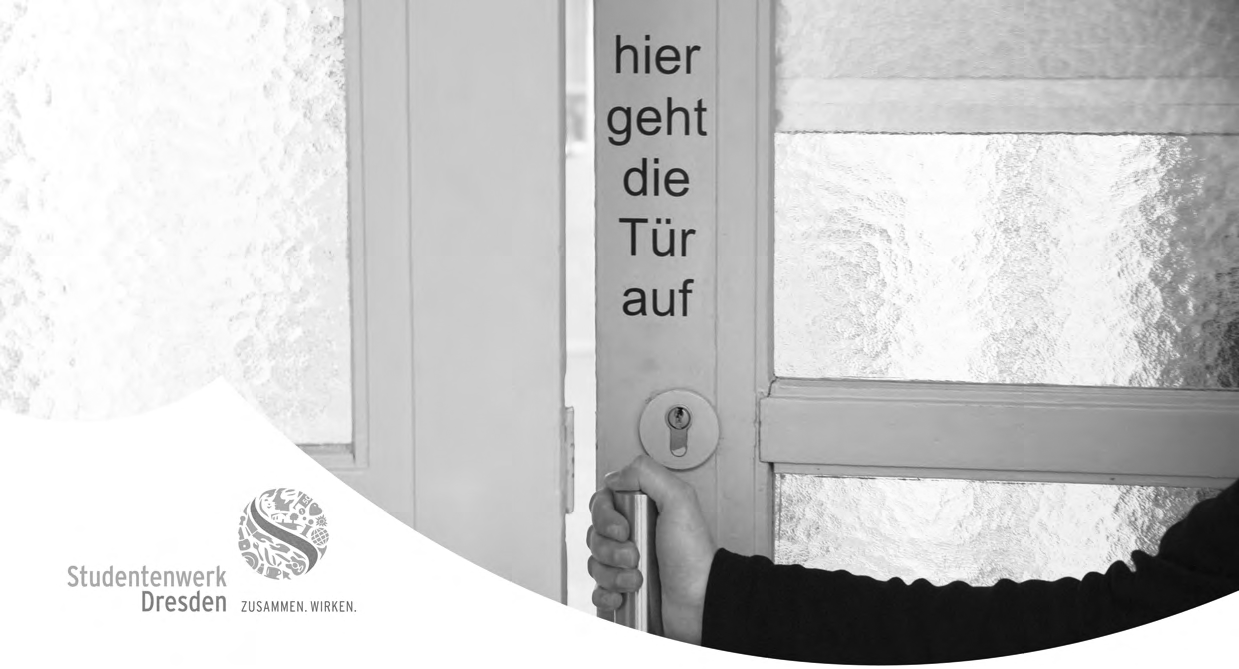
\includegraphics[width=\textwidth]{./psychoberatung-titlepicture-gray.png}

\section*{Psychosoziale Beratung für Studierende}
\label{sec:psychosoziale_beratung_fur_studierende}
Die Zeit des Studiums ist eine Phase der Persönlichkeitsentwicklung, die nahezu 
gesetzmäßig mit Krisen verbunden ist. Bereiche des psychologischen Beratungsbedarfs können z. B.\ sein:
\begin{itemize}
  \item  Zweifel, das Studium fortzusetzen oder Studienabschlussprobleme
  \item Arbeitsschwierigkeiten 
\item Prüfungsang
   \item      Prüfungsangst
  \item    psychosomatische Beschwerden
\item  mangelndes Selbstwertgefühl
\item Probleme mit Alkohol, Drogen, Online-Sucht
\item    depressive Verstimmungen
\item   Probleme mit dem sozialen Umfeld
\item   Bei Partnerschaftsproblemen ist auch Paarberatung möglich
\end{itemize}
\keyword{Psychosoziale Beratungsstelle (PSB)}:
\label{sub:psychosoziale_beratungsstelle_psb_}
Leiterin: Dr. Sabine Stiehler, 
Schnorrstraße 8, 01069 Dresden

Sie können folgende Kontaktmöglichkeiten zur Terminvereinbarung nutzen:
\begin{description}
  \item[Offene Sprechstunde] Dienstag 10--11h und Donnerstag 13--14h
  \item [E-Mail] psb@studentenwerk-dresden.de
  \item [Telefon] 0351 4697-920    
\end{description}
Weitere Informationen und das Seminarangebot der PSB finden Sie unter: \url{http://swdd.eu/psb}

